%!TEX root = ../thesis.tex

\section{課題点と2つのアプローチによる実験}
我々が行ってきた研究では, 簡易的なシミュレータ上で提案手法が有効だと確認されている. そのため, 次の段階として実環境における提案手法の有効性を検証することを試みた. そこで, 新たに顕在化した課題点は以下の2つの点である.

\begin{itemize}
  \item 実験条件(主にカメラ画像に影響を及ぼす光である)を揃える関係上, 実験を行う時間帯を光の変化が少ない夜間に固定する必要があるため, 1日に実験を行える時間が少なく, 1回の学習に何日も費やす必要がある
  \item 長時間の学習に耐えられるだけのバッテリ容量がロボットにない
\end{itemize}

これらの課題点から, 学習時間の短縮が必要であると判断した. そのため, 2つのアプローチを提案し, 学習量を削減する.
\par
この節では, まず, 従来の実験を簡単に紹介する. 次に, 2つのアプローチについての詳細と行った実験を述べる. 最後に, アプローチを試みる前と各アプローチによる実験結果を比較し, 議論を行う.

\subsection{従来の実験}

\begin{itemize}
  \item 実験目的\\
  簡易的なシミュレータ上で, 提案手法の有効性の検証を行う
  \item 実験環境\\
  4.1.1で述べた簡易的なシミュレータ環境で実験を行った
  \item 実験方法\\
  4.1.2で示した経路を繰り返し走行させる. 学習を60000step実行後, テストフェーズに移行する. テストフェーズで正しい順序で経路を選択し, 走行を行えるか確認する. この一連の流れを10回繰り返し行う.

  \newpage

  \item 実験結果\\
  実験結果を\figref{Fig:60000step}に示す. この図は, それぞれの走行パターンにおいて正しく経路を選択し, 走行できた回数を表している. \tabref{table:result}に全パターンを合計した結果を示す. なお, 分母が120であるのはテストフェーズにおいて, 全12パターンからなる経路を走行させ, 評価を行うことを10回繰り返したためである. 
  \par
  \tabref{table:result}に示すように, 目標方向に従って113/120回, 正しい経路を選択する様子が見られた. 

\begin{figure}[hbtp]
  \centering
 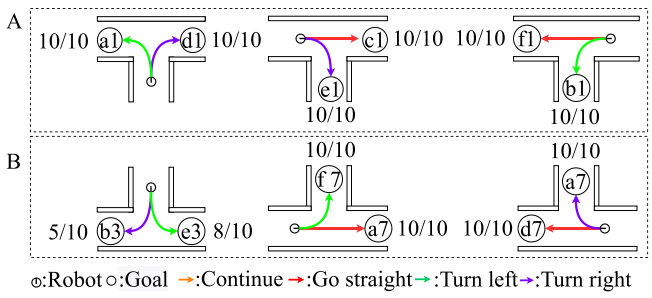
\includegraphics[keepaspectratio, scale=0.5]
      {images/60000step.png}
 \caption{Experimental results for each moving pattern from \cite{mech}}
 \label{Fig:60000step}
\end{figure}


\begin{table}[hbtp]
  \caption{Experimental results}
  \label{table:result}
  \centering
  \begin{tabular}{|c|c|c|}
    \hline
    Experiments & Step & Total result\\
    \hline
    Conventional & 60000 & 113/120(94.2\%)\\
    \hline
  \end{tabular}
\end{table}

\end{itemize}

\subsection{アプローチ1:データセットの割合変更}

\begin{itemize}
  \item 
\end{itemize}

% \begin{figure}[hbtp]
%   \centering
%  \includegraphics[keepaspectratio, scale=0.8]
%       {images/RaspberryPiMouse.png}
%  \caption{Example}
%  \label{Fig:Example}
% \end{figure}

\newpage
